\documentclass[14pt]{article}
\usepackage[margin=1in]{geometry}
\usepackage{amsmath}
\usepackage{amssymb}
\usepackage{fancyhdr}
\usepackage{graphicx}
\usepackage{xcolor}
\usepackage{hyperref}
\renewcommand{\familydefault}{\sfdefault}
\parindent 0ex
\everymath{\displaystyle{}}

\begin{document}
    \begin{center}
        \textbf{Math 275 Notes\\ Calculus For Engineers and Scientists\\Andy Smit}
    \end{center}
    \section{Derivatives}
    \textbf{Derivative of a Function: }\\
    A function $f$ is said to have a derivative at a real number $c$ if \\$\lim \limits_{h\rightarrow 0} \frac{f(c+h)-f(c)}{h}$ exists
    \\\\
    \textbf{An Alternative Definition of the Derivative:}
    $$f'(x)=\lim \limits_{x \rightarrow c} \frac{f(x)-f(c)}{x-c}$$
    \textbf{Differentiable Function:}\\
    A function $f$ is said to be differentiable at $c$ if $f'(x)$ exists. However if $f'(c)$ does not not exist, one says $f$ is not differentiable at $c$.
    \\\\
    \textbf{Other Notations for Derivatives:}\\
    Given $y=f(x)$, the derivative may be denoted by
    \begin{enumerate}
        \item $f'(x)$
        \item $y'$
        \item $\frac{dy}{dx}$
        \item $\frac{d}{dx} \Big\{f(x)\Big\}$
    \end{enumerate}
    \textbf{Function Notation:}\\
    Let $f$ and $g$ be given functions
    \begin{enumerate}
        \item Sum: $(f+g)(x)=f(x)+g(x)$
        \item Difference: $(f-g)(x)=f(x)-g(x)$
        \item Constant Multiple: $(k\, f)(x)=k\,f(x)$
        \item Product: $(f\,g)(x)=f(x)g(x)$
        \item Quotent: $\bigg(\frac{f}{g}\bigg)(x)=\frac{f(x)}{g(x)}$
        \item Composition: $(f \circ g)(x)=f(g(x))$
    \end{enumerate}
    \textbf{The Power Rule:}
    $$\frac{d}{dx}\Big(x^n \Big)=n\,x^{n-1} $$
    \textbf{Derivative Rules:}\\
    Let $f$, $g$, $u$ and $v$ be differentiable functions and $k$ be a constant:
    \begin{enumerate}
        \item Sum/Difference Rules: $\frac{d}{dx}\Big(f(x)\pm g(x)\Big)=\frac{d}{dx}\Big(f(x)\Big)\pm\frac{d}{dx}\Big(g(x)\Big)$
        \item Constant Multiple: $\frac{d}{dx}\Big(k\, f(x)\Big)=k\, \frac{d}{dx}\Big(f(x)\Big)$
        \item Product Rule: $\frac{d}{dx}\Big(u\,v\Big)=v\frac{d}{dx}\Big(u\Big)+u\frac{d}{dx}\Big(v\Big)= v\,u'+u\,v'$
        \item Quotent Rule: $\frac{d}{dx}\Big(\frac{u}{v}\Big)=\frac{v\frac{d}{dx}\big(u\big)-u\frac{d}{dx}\big(v\big)}{v^2}=\frac{v\,u'-u\,v'}{v^2}$
        \item Chain Rule: $\frac{d}{dx}\Big(f(u)\Big)=f'(u)\,\frac{du}{dx}$
    \end{enumerate}
    \textbf{Geometric Interpretation of the Derivative:}
    Let $y=f(x)$ be a differentiable function at $c$, and let $P(c, f(c))$, and $Q(x,y)=Q(x, f(x))$ be points on its graph as shown:\\
    \textcolor{red}{Secant Line: A straight line joining any 2 points $P$, and $Q$ on $f(x)$}\\
    \textcolor{blue}{Tangent Line: A straight line that touches $f(x)$ at point $P$}\\
    \textcolor{green}{Normal Line: A straight line perpendicular to the tangent line of $f(x)$ at point $P$}\\
    \includegraphics[width=\textwidth]{fig1.png}\\
    \textbf{The Slope of a Tangent Line:}\\
    Let $y=f(x)$ be a differentiable function at point $c$. Then the slope of the tangent line of $f$ at $c$ is $$\left. m_{tan}\right|_{x=c}=f'(c)$$
    \textbf{Equation of a Straight Line:}\\
    Point Slope Form: An equation of the straight line passing through the point $P(x,y)$, and has slope $m$ is of the form $$y-y_0=m(x-x_0)$$
    \textbf{Higher Order Derivatives}\\
    Let $f$ be a differentiable function, that $f'(x)$ exists. From now on we may call $f'(x)$ the first order derivative of $f$. Assume $f$ is still differentiable. The second order derivative is defined as: $$\frac{d}{dx}\left\{f'(x)\right\}=f''(x)$$
    \textbf{Continuity at a Point}\\
    A function $f$ is said to be continuous at $c$ if the following the conditions hold: 
    \begin{enumerate}
        \item $f'(c)$ is defined and real
        \item $\lim \limits_{x\rightarrow c} f(x)=L$ where $L$ is a real, non infinite number.
        \item $\lim \limits_{x\rightarrow c} f(x)=f(c)$
    \end{enumerate}
    If any of the above conditions are not satisfied then $f$ is not continuous at $c$.\\\\
    \textbf{Left and Right Hand Derivatives:}
    Let $f(x)$ be a given function.
    \begin{enumerate}
        \item The left-hand derivative of $f$ at $c$ is denoted and defined by $$f_-'(c)=\lim \limits_{x\rightarrow c^-} \frac{f(x)-f(c)}{x-c}$$ provided the limit exists.
        \item The right-hand derivative of $f$ at $c$ is denoted and defined by $$f_+'(c)=\lim \limits_{x\rightarrow c^+} \frac{f(x)-f(c)}{x-c}$$ provided the limit exists.
    \end{enumerate}Both the left and right hand derivatives may not exist.\\\\
    \textbf{Differentiability and Left and Right hand derivatives:}\\
    Let $f$ be a given function
    \begin{enumerate}
        \item If left and right hand derivatives of $f$ at $c$ exist and are equal then $f$ is differentiable at $c$, and that $f'(c)=f_-'(c)=f_+'(c)$.
        \item If either the left or right hand derivatives of $f$ at $c$ do not exist or both exist but are not equal, then $f$ is not differentiable at $c$ and $f'(c)$ does not exist.
    \end{enumerate}
    \textbf{Relationship between Differentiability and Continuity:}
    Let $f$ be a given function. If $f$ is differentiable at $c$, then $f$ is necessarily continuous at c.
    \begin{itemize}
        \item If $f$ is differentiable at $c$ then $f$ must be continuous
        \item If $f$ is discontinuous at $c$ then $f$ is not differentiable
        \item The converse of the theorem is not true.
    \end{itemize} 
    \textbf{Easy way to calculate The left and Right Hand Derivative:}\\
    Let $f$ be a given function continuous at $c$.
    \begin{enumerate}
        \item $f_-'(c)=\lim \limits_{x \rightarrow c^-}f(x)$
        \item $f_+'(c)=\lim \limits_{x \rightarrow c^+}f(x)$
    \end{enumerate}
    \section{Special Functions}
    \textbf{The Derivatives of the Six Trigonometric Functions:}
    \begin{enumerate}
        \item \begin{enumerate}
            \item $\lim \limits_{h\rightarrow0} \frac{\sin(h)}{h}=1$
            \item $\lim \limits_{h\rightarrow0} \frac{\cos(h)}{h}=0$
        \end{enumerate}
        \item \begin{enumerate}
            \item $\frac{d}{dx}\Big(\sin(x)\Big)=\cos(x)$
            \item $\frac{d}{dx}\Big(\cos(x)\Big)=-\sin(x)$
        \end{enumerate}
        \item \begin{enumerate}
            \item $\frac{d}{dx}\Big(\tan(x)\Big)=\sec^2(x)$
            \item $\frac{d}{dx}\Big(\cot(x)\Big)=-\csc^2(x)$
        \end{enumerate}
        \item \begin{enumerate}
            \item $\frac{d}{dx}\Big(\sec(x)\Big)=\sec(x)\tan(x)$
            \item $\frac{d}{dx}\Big(\csc(x)\Big)=-\csc(x)\cot(x)$
        \end{enumerate}
    \end{enumerate}
    \subsection{Inverse Functions}
    \textbf{A Function of a Single Read Number:}\\
    A function $f$ is a rule that assigns to each permissible real number $x$, one and only one real number $y$. $$y=f(x)$$
    \textbf{Vertical Line Test for the Graph of a Function:}\\
    Every vertical line cuts the graph of a function at most once.\\\\
    \textbf{Properties of the Graph of a Function:}\\
    The graph of a function can be used as a tool which enables us to obtain $y$ from a given $x$.\\
    It is possible that $f(x_1)=f(x_2)=y$ for $x_1\neq x_2$. If the function $f(x)$ has no points $x_1\neq x_2$ such that $f(x_1)=f(x_2)$ it is said to be an invertible function. 
    The inverse of $f$ is denoted $g$ or $f^{-1}$. $f^{-1}$ takes the $y$ value back to $x$.\\ 
    $f(x)=y$ and $f^{-1}(y)=x$ are equivalent.\\\\
    \textbf{Conversion Rules:}\\
    To convert one statement to the other simply move $f$ from one side to the other as $f^{-1}$ and vice versa.
    $$f(x)=y \Leftrightarrow f^{-1}(y)=x$$
    \textbf{One To One Functions:}\\
    Let $f$ be a given function on $[a,b]$\\
    The function $f$ is said to be one to one on $[a,b]$ if every horizontal and vertical line cuts the graph of the function at most once.
    \begin{itemize}
        \item A function may not be one to one on $[a,b]$, however $[a,b]$ may be restricted so that the function is one to one.
        \item Important Examples of one to one functions\begin{enumerate}
            \item Strictly Increasing functions ($f'(x)>0$, $x\in[a,b]$)
            \item Strictly Difference function ($f'(x)<0$, $x\in[a,b]$)
        \end{enumerate}
    \end{itemize}
    \textbf{One to One Functions and the Inverse}\\
    Let $f$ be a given function defined on $[a,b]$. If $f$ is one to one on $[a,b]$, then $f$ is invertible on $[a,b]$, meaning $f^{-1}$ exists.\\\\
    \textbf{A Formula for the Inverse Function:}\\
    Let $f$ be a given function and assume $f$ has an inverse. To find a formula for $y=f^{-1}(x)$:
    \begin{enumerate}
        \item Interchange $x$ and $y$. $x\leftrightarrow y$
        \item Solve for $y$ as a function of $x$
    \end{enumerate}
    If an explicit inverse does not exist, leave in an implicit form.\\\\
    \textbf{The Derivative of the Inverse Function:}\\
    Let $y=f(x)$ be a given function. Assume $f$ has an inverse. Then 
    $$\frac{d}{dx}\Big(f^{-1}(c)\Big)=\frac{1}{f'\Big(f^{-1}\big(c\big) \Big)}$$
    \textbf{Properties of Inverse Functions:}\\
    \begin{enumerate}
        \item The domain of $f$ coincide with the range of $f^{-1}$ and vice versa.
        \item Cancellation Properties \begin{enumerate}
            \item $f^{-1}\Big(f(x)\Big)=x$ for all $x$ in the range of $f$.
            \item $f\Big(f^{-1}(x)\Big)=x$ for all $x$ in the range of $f$.
        \end{enumerate} 
        \item The graph $y=f^{-1}(x)$ is the reflection in the line $y=x$ of the graph $y=f(x)$
    \end{enumerate}
    \subsection{Exponential and Logarithmic Functions}
    \textbf{The Natural Number $e$:}
    The natural number $e$ is denoted and defined by, \\
    \begin{center}
        $e=\lim \limits_{x\rightarrow0} (1+x)^{\frac{1}{x}}$ or $e=\lim \limits_{x\rightarrow\infty}\left(1+\frac{1}{x}\right)^x$
    \end{center} 
    An estimate for $e\approx2.718$\\\\
    \textbf{Special Exponential Function:}\\
    Consider the exponential function $y=a^x$.\\
    If $a=e$, then $y=e^x$, which is called the natural exponential function.\\\\
    \textbf{Two Special Logarithms:}\\ 
    Consider the logarithmic function $y=\log(x)$.\\
    If base $a=10$, then $y=\log_10(x)$, which is called the common logarithm.\\
    If base $a=e$, then $y=\log_e(x)$, which is called the natural logarithm and is denoted $y=\ln(x)$.\\\\
    \textbf{Properties of Logarithms:}\\
    \begin{tabular}{p{5cm}p{5cm}}
        L1: $\log_a(x)+\log_a(y)=\log_a(x\,y)$ & L2:$\log_a(x)-\log_a(y)=\log_a\left(\frac{x}{y}\right)$\\
        L3: $\log_a\left(x^n\right)=n \log_a(x)$& L4: $\log_a(1)=0$\\
        L5: $\log_a (a)=1 \leftrightarrow a^1=a$& L6: $\log_a\left(a^x\right)=x$\\
        L7: $log_b(x)=\frac{\log_a(x)}{\log_a(b)}$& 
    \end{tabular}\\\\
    \textbf{Derivatives of Exponential and Logarithmic Functions:}\\
    \begin{itemize}
        \item $\frac{d}{dx} e^x=e^x$
        \item $\frac{d}{dx} \ln(x)=\frac{1}{x}$
        \item $\frac{d}{dx} a^x=a^x\ln(x)$
        \item $\frac{d}{dx} \log_a(x)=\frac{1}{x\ln(a)}$
    \end{itemize}
    \textbf{Logarithmic Differentiation:}
    \begin{itemize}
        \item Take natural Logarithm of both sides of an equation and simplify using the properties of logarithms.
        \item Take the derivative of both sides of the equation with respect to $x$
    \end{itemize}
    $y=f(x)$\\
    $\ln(y)=\ln(f(x))$\\
    $\frac{1}{y} \frac{dy}{dx} = \frac{f'(x)}{f(x)}$\\
    $\frac{dy}{dx}=f'(x)$
    \subsection{Inverse Trigonometric Functions}
    Inverse Sine Function: $\sin^{-1}(x)$ or $\arcsin(x)$ $\mathrm{D}\in(-1,1)$ $\mathrm{R}\in\left(-\frac{\pi}{2},\frac{\pi}{2}\right)$\\
    Inverse Cosine Function: $\cos^{-1}(x)$ or $\arccos(x)$ $\mathrm{D}\in(-1,1)$ $\mathrm{R}\in(0, \pi)$\\
    Inverse Tangent Function: $\tan^{-1}(x)$ or $\arctan(x)$ $\mathrm{D}\in(-\infty,\infty)$ $\mathrm{R}\in\left(-\frac{\pi}{2},\frac{\pi}{2}\right)$\\
    Inverse Cosecant Function: $\csc^{-1}(x)$\\
    Inverse Secant Function: $\sec^{-1}(x)$\\
    Inverse Cotangent Function: $\cot^{-1}(x)$\\
    \textbf{Derivatives of Inverse Trigonometric Functions:}\\
    \begin{tabular}{p{5cm}p{5cm}}
        i. $\frac{d}{dx}\sin^{-1}(x)=\frac{1}{\sqrt{1-x^2}}$ & ii. $\frac{d}{dx}\cos^{-1}(x)=-\frac{1}{\sqrt{1-x^2}}$\\
        iii. $\frac{d}{dx}\tan^{-1}(x)=\frac{1}{1+x^2}$ & iv. $\frac{d}{dx}\cot^{-1}(x)=-\frac{1}{1+x^2}$\\
        v. $\frac{d}{dx}\sec^{-1}(x)=\frac{1}{|x|\sqrt{x^2-1}}$ & vi. $\frac{d}{dx}\sec^{-1}(x)=\frac{1}{|x|\sqrt{x^2-1}}$
    \end{tabular}\\\\
    \textbf{Properties of Inverse Trigonometric Functions:}\\
    Group A\\
    \begin{tabular}{p{5cm}|p{5cm}}
        (i) $\sin(-x)=-\sin(x)$ & $\sin^{-1}(-x)=-\sin^{-1}(x)$\\
        (ii) $\tan(-x)=-\tan(x)$ & $\tan^{-1}(-x)=-\tan^{-1}(x)$\\
        (ii) $\cos(-x)=\cos(x)$ & $\cos^{-1}(-x)=\pi-\cos^{-1}(x)$
    \end{tabular}\\
    Cancellation Properties\\
    \begin{tabular}{p{6cm}|p{5cm}}
        (i) $\sin(\sin^{-1}(x))=x$, $x\in[-1,1]$ & $\sin^{-1}(\sin(y))=y$, $y\in\left[-\frac{\pi}{2}, \frac{\pi}{2}\right]$\\
        (ii) $\tan(\tan^{-1}(x))=x$, $x\in(-\infty,\infty)$ & $\tan^{-1}(\tan(y))=y$, $y\in\left[-\frac{\pi}{2}, \frac{\pi}{2}\right]$\\
        (iii) $\cos(\cos^{-1}(x))=x$, $x\in[-1,1]$ & $\cos^{-1}(\cos(y))=y$, $y\in\left[0, \pi\right]$\\
    \end{tabular}\\
    The function $\sin(x)$ and $\cos(x)$ are periodic with periods of $2\pi$\\
    The function $\tan(x)$ is periodic with period $\pi$. 
    \subsection{Hyperbolic Functions}
    The hyperbolic functions are combinations of the exponential function, and have properties very similar to that of the trigonometric functions.\\
    \textbf{The 6 Hyperbolic Functions:}\\
    \begin{enumerate}
        \item The Hyperbolic Sine Function: $$\sinh(x)=\frac{e^x-e^{-x}}{2}$$
        \item The Hyperbolic Cosine Function: $$\cosh(x)=\frac{e^x+e^{-x}}{2}$$
        \item The Hyperbolic Tangent Function: $$\tanh(x)=\frac{\sinh(x)}{\cosh(x)}=\frac{e^x-e^{-x}}{e^x+e^{-x}}$$
        \item The Hyperbolic Cosecant Function: $$\mathrm{csch}(x)=\frac{1}{\sinh(x)}=\frac{2}{e^x-e^{-x}}$$
        \item The Hyperbolic Secant Function: $$\mathrm{sech}(x)=\frac{1}{\cosh(x)}=\frac{2}{e^x+e^{-x}}$$
        \item They Hyperbolic Cotangent Function: $$\mathrm{coth}(x)=\frac{1}{\tanh(x)}=\frac{\cosh(x)}{\sinh(x)}=\frac{e^x+e^{-x}}{e^x-e^{-x}}$$
    \end{enumerate}
    \textbf{The Hyperbolic Identities and Properties:}
    \begin{enumerate}
        \item $\cosh^2(x)-\sinh^2(x)=1$
        \item $\cosh(x)+\sinh(x)=e^x$
        \item $\cosh(x)-\sinh(x)=e^{-x}$
    \end{enumerate}
    \textbf{Derivative of the Hyperbolic Functions:}\\
    \begin{enumerate}
        \item $\frac{d}{dx} \sinh(x)=\cosh(x)$
        \item $\frac{d}{dx} \cosh(x)=\sinh(x)$
        \item $\frac{d}{dx} \tanh(x)=\mathrm{sech}^2(x)$
        \item $\frac{d}{dx} \mathrm{coth}(x)=-\mathrm{csch}^2(x)$
        \item $\frac{d}{dx} \mathrm{sech}(x)=-\mathrm{sech}(x)\tanh(x)$
        \item $\frac{d}{dx} \mathrm{csch}(x)=-\mathrm{csch}(x)\mathrm{coth}(x)$
    \end{enumerate}
    \textbf{Inverse Hyperbolic Functions:}\\
    \begin{enumerate}
        \item Inverse Hyperbolic Sine Function: $\mathrm{D}\in(-\infty, \infty)$ $\mathrm{R}\in(-\infty, \infty)$
        $$\sinh^{-1}(x)=\ln(x+\sqrt{x^2+1}) $$
        \item Inverse Hyperbolic Cosine Function: $\mathrm{D}\in[1, \infty)$ $\mathrm{R}\in[0, \infty)$
        $$\cosh^{-1}(x)=\ln(x+\sqrt{x^2-1})$$
        \item Inverse Hyperbolic Tangent Function: $\mathrm{D}\in(-1, 1)$ $\mathrm{R}\in(-\infty, \infty)$
        $$\tanh^{-1}(x)=\frac{1}{2}\ln\left(\frac{1+x}{1-x}\right)$$
        \item Inverse Hyperbolic Cotangent Function: $\mathrm{D}\in(-\infty, -1)\cup(1, \infty) $ $\mathrm{R}\in(-\infty,0)\cup(0, \infty)$
        $$\mathrm{coth}^{-1}(x)=\frac{1}{2}\ln\left(\frac{x+1}{x-1}\right)$$
        \item Inverse Hyperbolic Secant Function: $\mathrm{D}\in(0, 1]$ $\mathrm{R}\in[0, \infty)$
        $$\mathrm{sech}^{-1}(x)=\ln\left(\frac{1}{x}+\sqrt{\frac{1}{x^2}-1}\right)$$
        \item Inverse Hyperbolic Cosecant Function: $\mathrm{D}\in(-\infty,0)\cup(0, \infty)$ $\mathrm{R}\in(-\infty,0)\cup(0, \infty)$
        $$\mathrm{csch}^{-1}(x)=\ln\left(\frac{1}{x}+\sqrt{\frac{1}{x^2}+1}\right)$$
    \end{enumerate}
    \textbf{Derivatives of Inverse Hyperbolic Functions:}\\
    \begin{tabular}{p{5cm}p{5cm}}
        i)$\frac{d}{dx}\sinh^{-1}(x)=\frac{1}{\sqrt{x^2+1}}$ & 
        ii) $\frac{d}{dx}\cosh^{-1}(x)=\frac{1}{\sqrt{x^2-1}}$\\
        iii)$\frac{d}{dx}\tanh^{-1}(x)=\frac{1}{1-x^2}$ & 
        iv) $\frac{d}{dx}\mathrm{coth}^{-1}(x)=\frac{1}{1-x^2}$\\
        v)$\frac{d}{dx}\mathrm{sech}^{-1}(x)=\frac{-1}{x\sqrt{1-x^2}}$ & 
        vi) $\frac{d}{dx}\mathrm{csch}^{-1}(x)=\frac{-1}{|x|\sqrt{1+x^2}}$\\
    \end{tabular}\\\\
    \section{Applications of Derivatives}
    \subsection{Error Estimation} 
    \textbf{Incremental Change of Independent and Dependent Variables:}\\
    Let $y=f(x)$. Assume that independent variable has changed from $x_0$ to $x$
    \begin{enumerate}
        \item The change of the independent variable is defined by $\Delta x=x-x_0$
        \item The change of the dependent variable is defined by $\Delta y=f(x)-f(x_0)$
    \end{enumerate}
    \textbf{Differentials of Independent and Dependent Variables:}\\
    Let $y=f(x)$. Assume that independent variable has changed from $x_0$ to $x$
    \begin{enumerate}
        \item The differential of the independent variable is denoted and defined by $dx=\Delta x$
        \item The differential of the dependent variable is denoted and defined by $dy=f'(x_0)\, dx$
    \end{enumerate}
    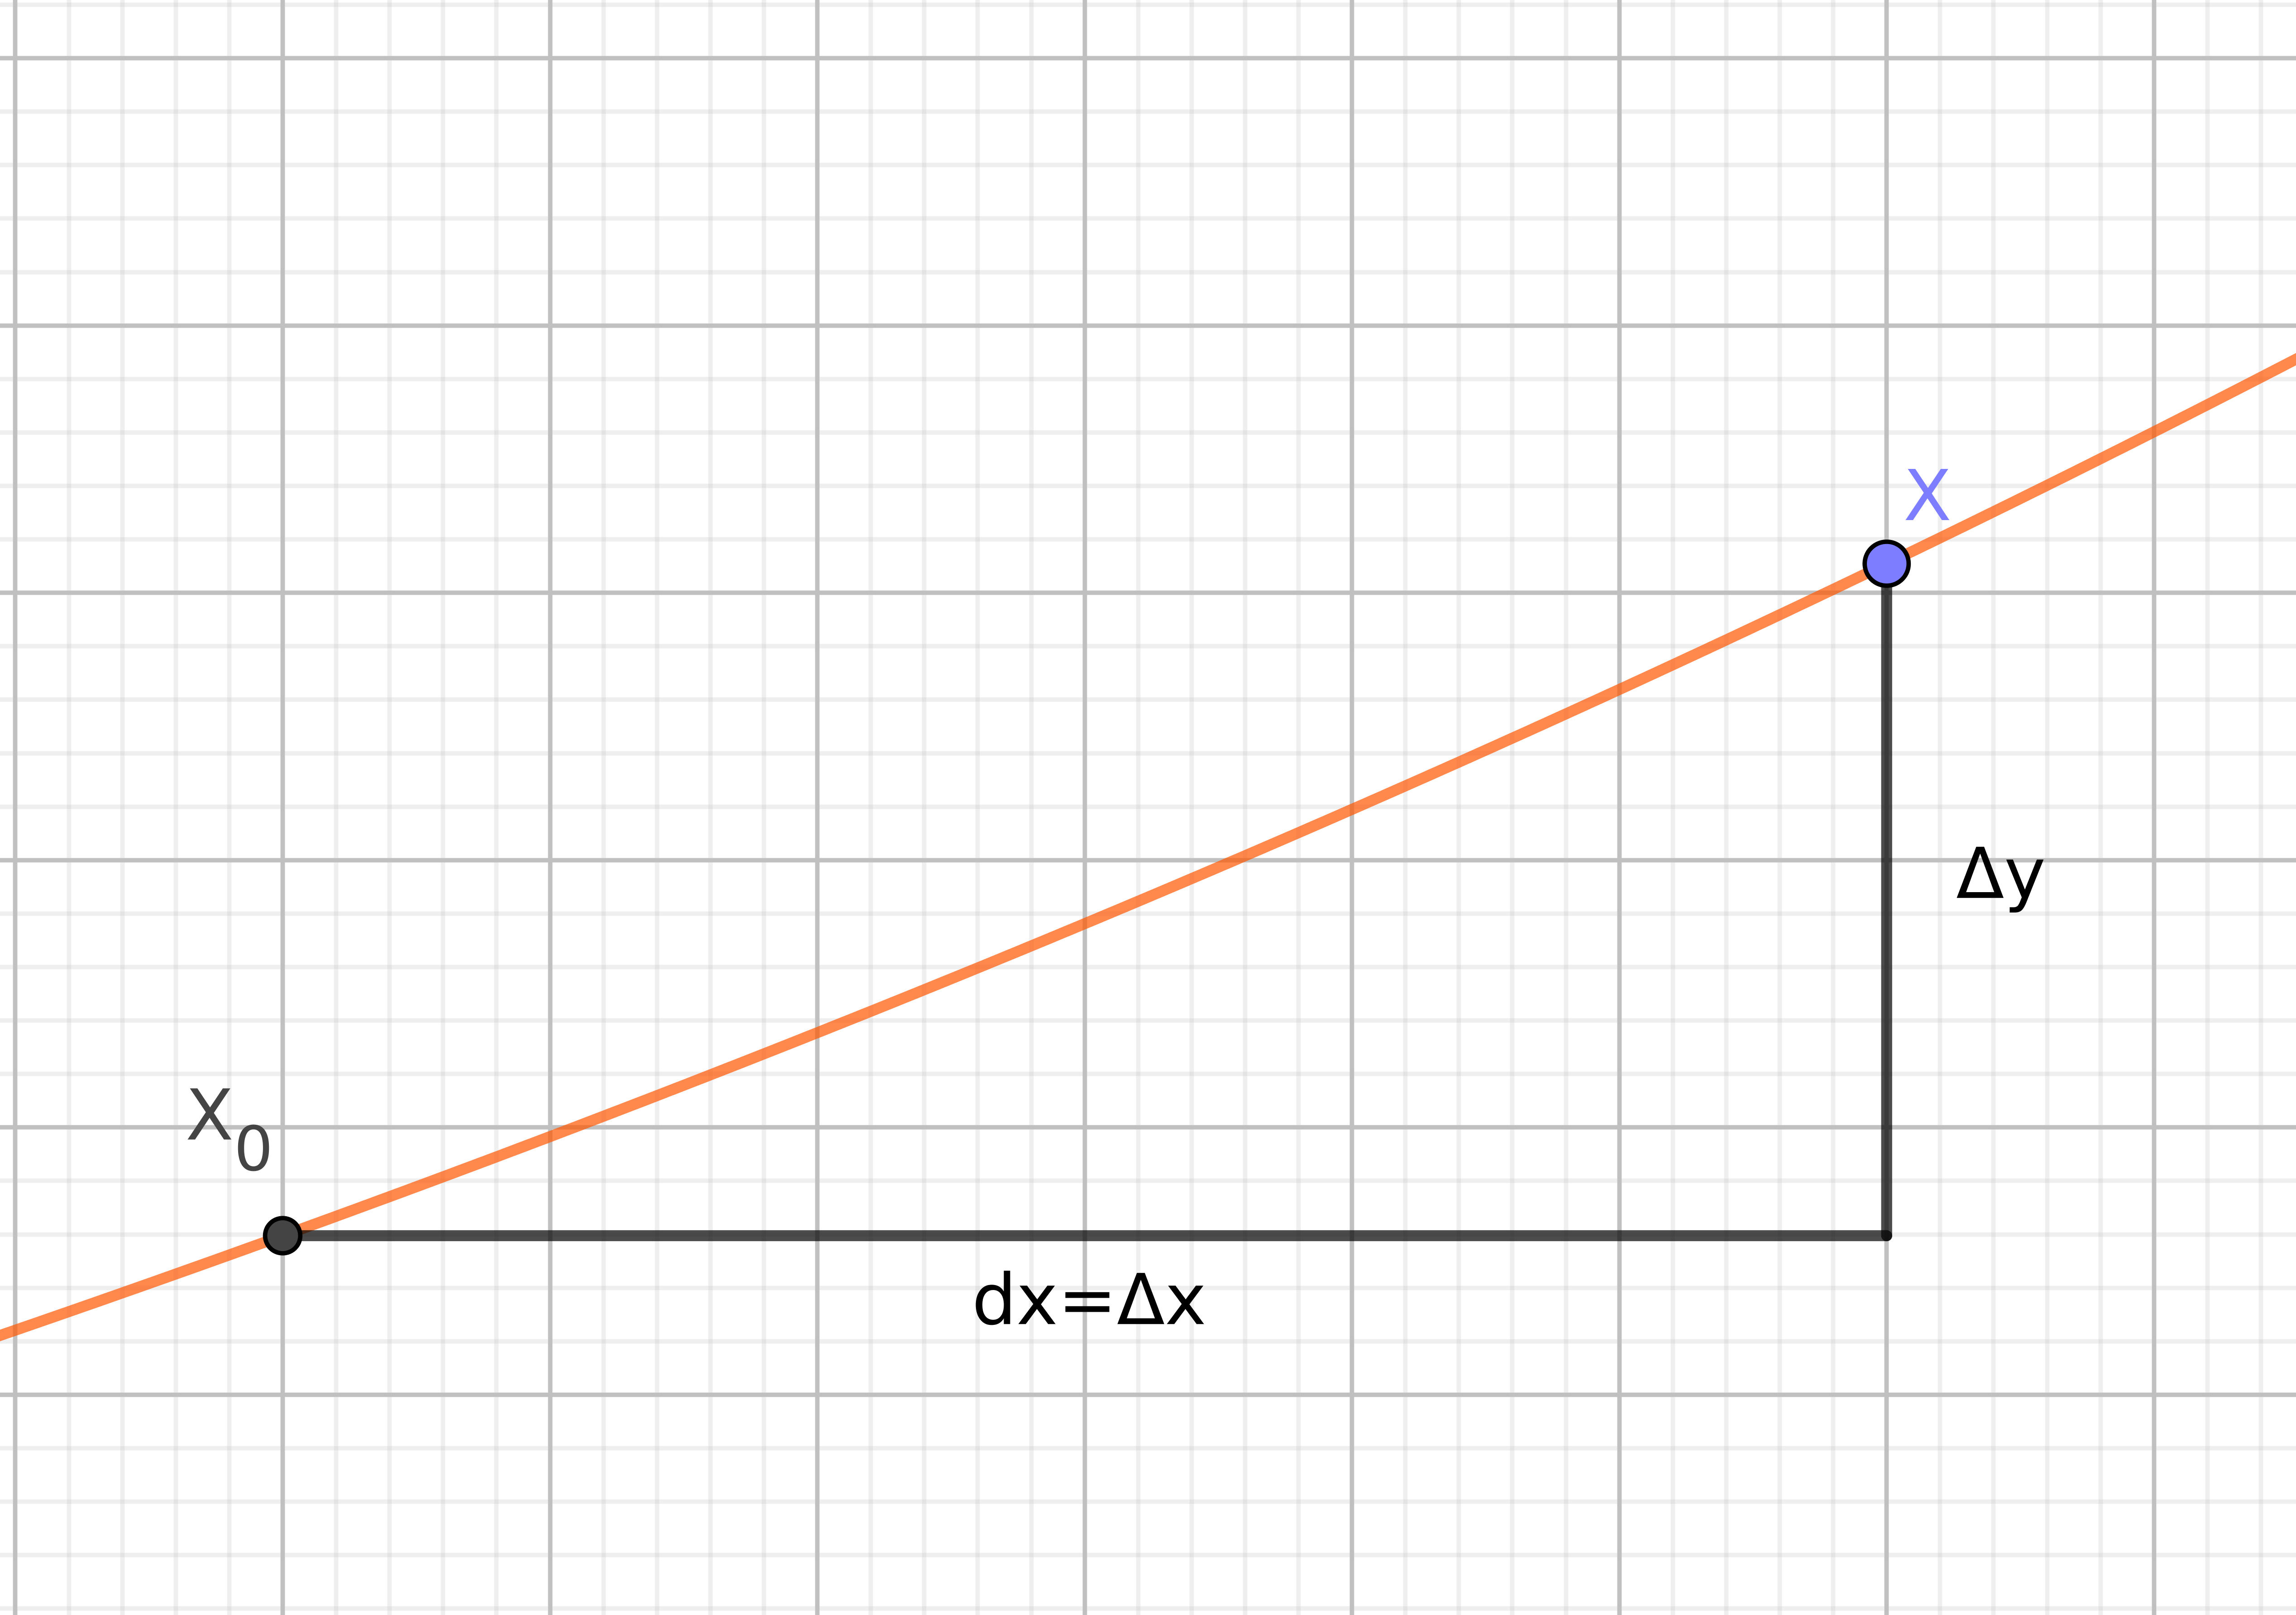
\includegraphics[width=0.5\textwidth]{differentials.png}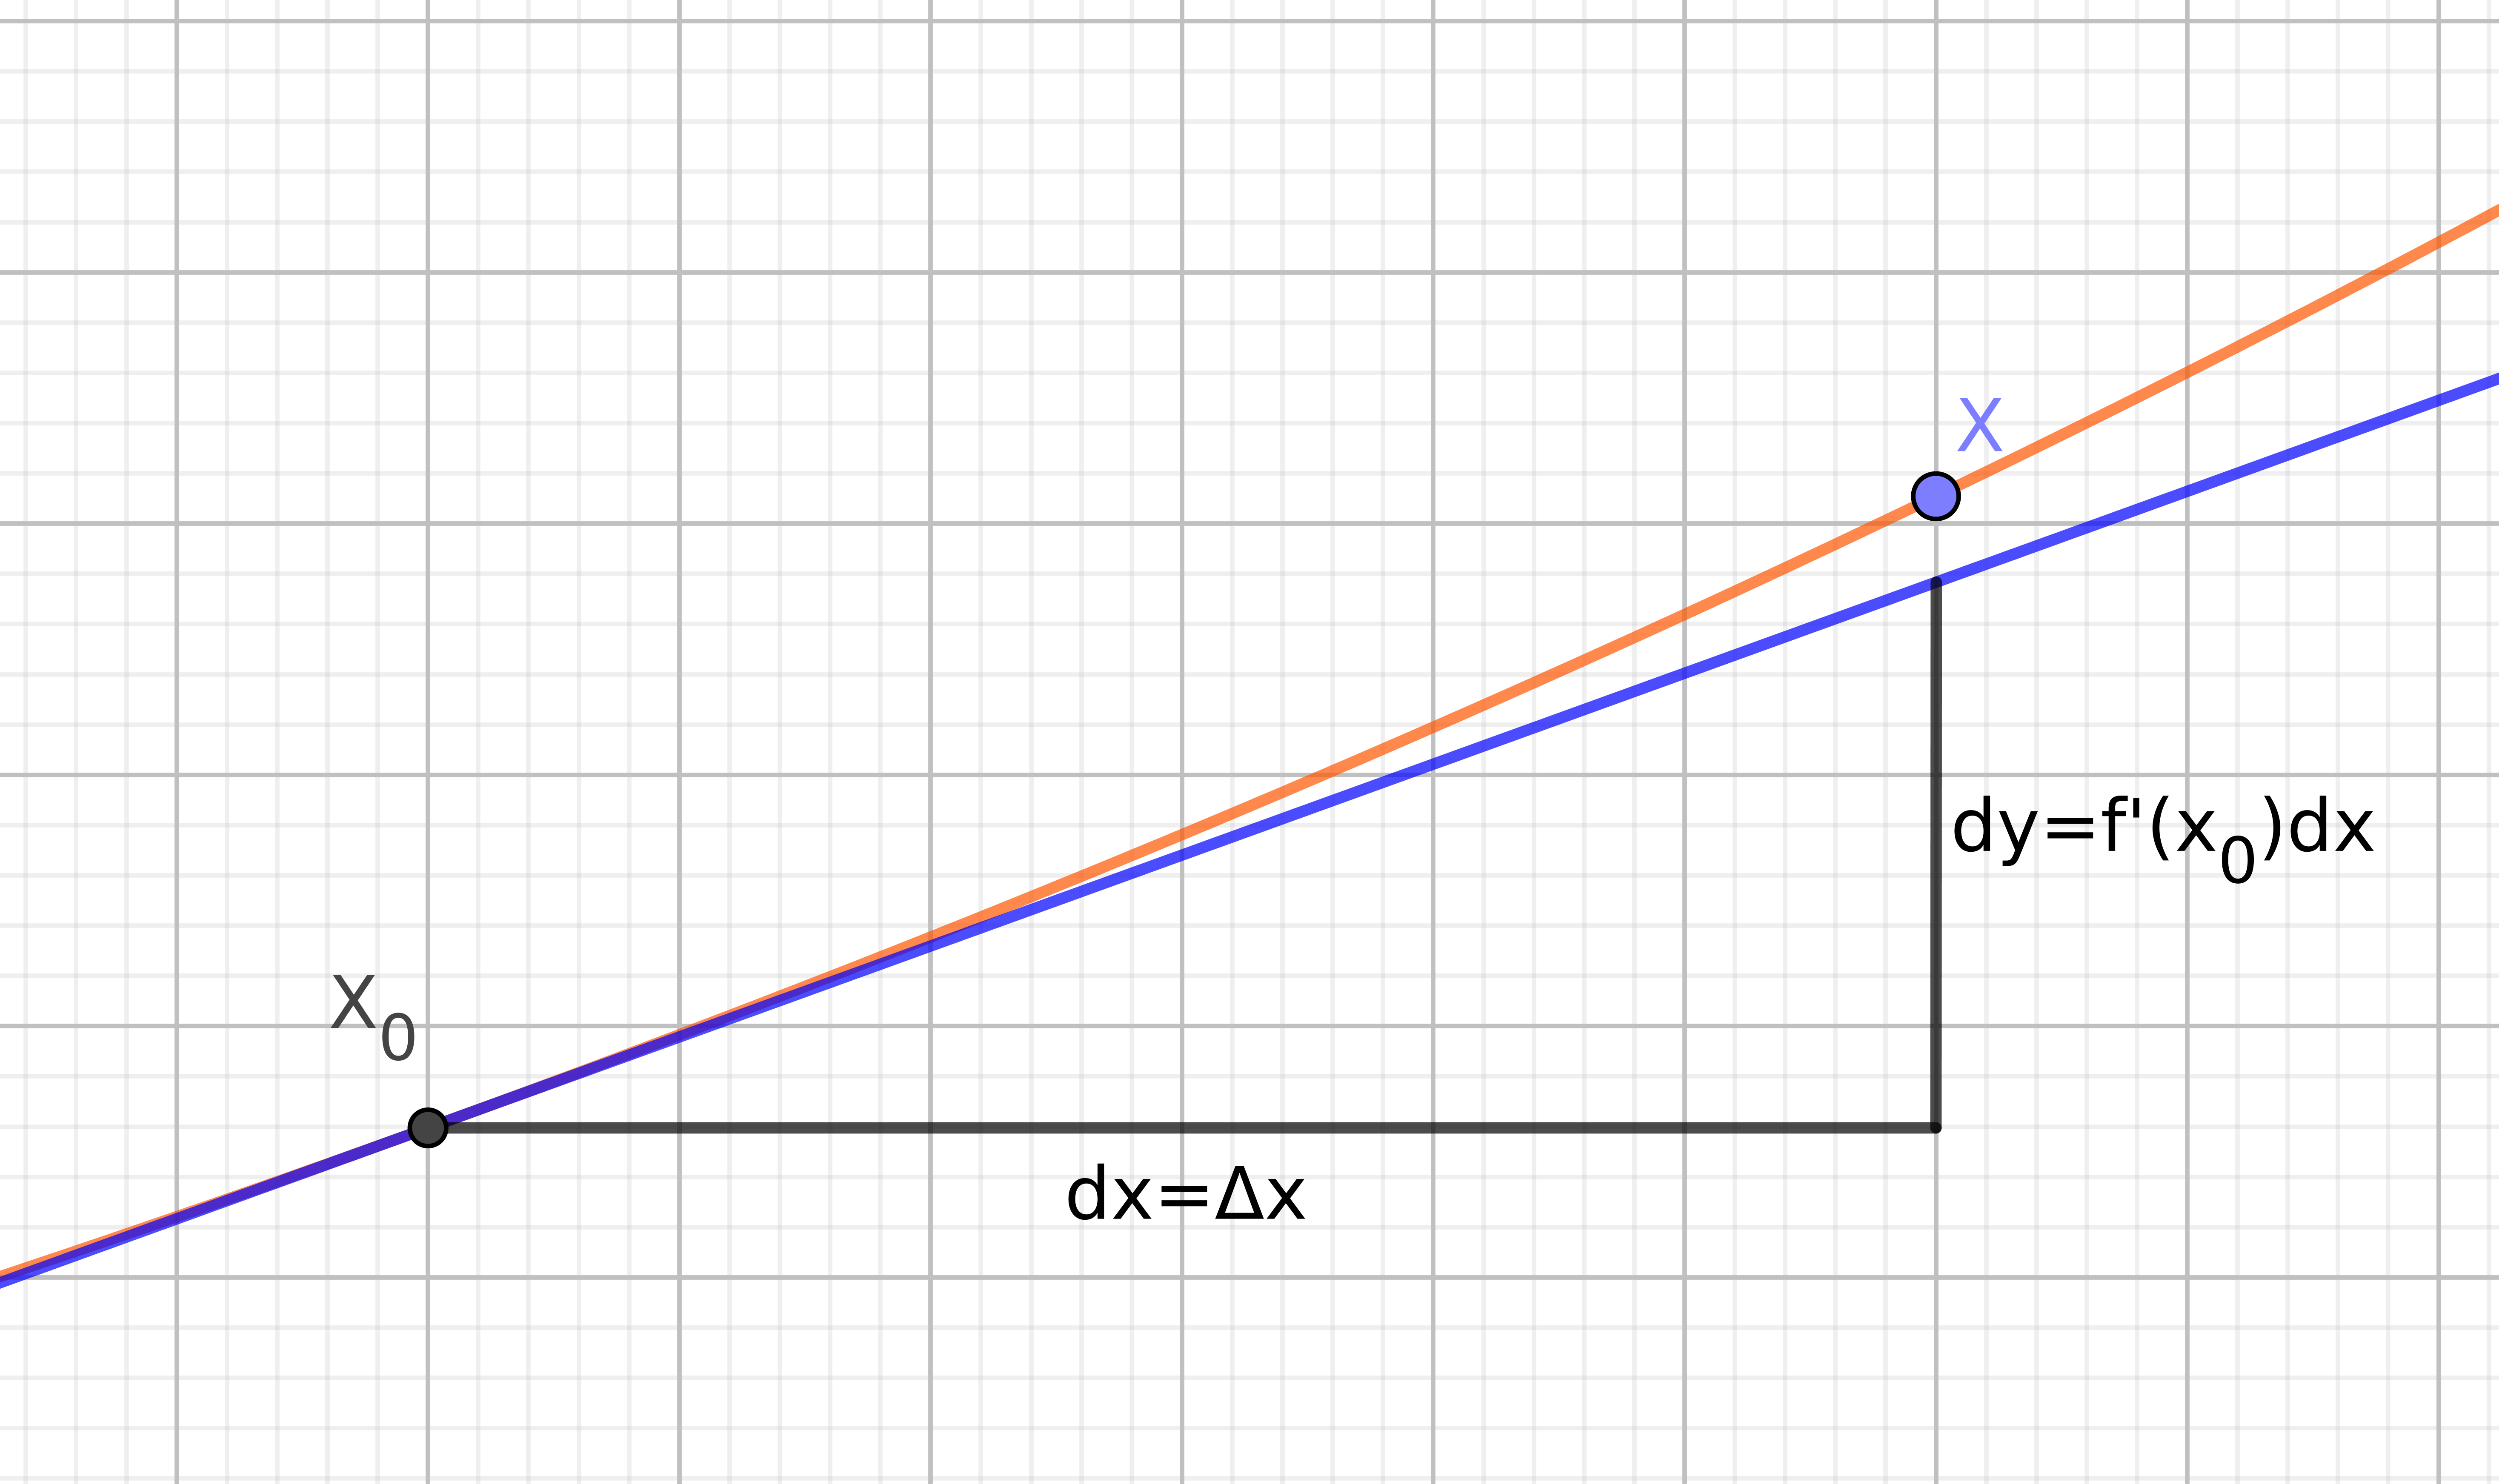
\includegraphics[width=0.5\textwidth]{differentials2.png}\\
    If the change in $x$ or $\Delta x$ is very small then $\Delta x$ may be thought of as the error in the measurement of $x$. Accordingly $\Delta y$ may be though of as the corresponding error in the measurement of $y$.\\
    \textbf{Relationship between $\Delta y$ and $dy$:}\\
    First observe $\Delta y$ is much more complicated then $dy$ to compute. If $\Delta x$ is small then $$\frac{\Delta y}{\Delta x}=\lim \limits_{\Delta x\rightarrow 0}\frac{f(x)-f(x_0)}{x-x_0}$$
    That is $\frac{\Delta y}{\Delta x}\approx\frac{dx}{dy}$ or $\Delta y\approx dy$\\\\
    \textbf{Classifying Error Types:}\\
    Assume a certain quantity has changed from $P_0$ to $P$. Then $\Delta P= P-P_0$.
    \begin{enumerate}
        \item Error: $\Delta P=P-P_0$
        \item Absolute Error: $|\Delta P|$
        \item Relative Error: $\frac{\Delta P}{P_0}$
        \item Percentage Error: $\frac{\Delta P}{P_0}\times 100\% $ 
    \end{enumerate}
    \subsection{Implicit Differentiation}
    \textbf{A Relation:}\\
    An equation with the independent variable $x$ and the dependent variable $y$ is a relation.\\\\
    \textbf{Explicit and Implicit Relations:}\\
    A relation is explicit, simply if and only if $y$ is expressed in terms of $x$. If a relation is not explicit then it is implicit.\\\\
    \textbf{Steps for Implicit Differentiation:}\\
    \begin{enumerate}
        \item Take the derivative of both sides of the relation with respect to $x$
        \item Group all terms containing $\frac{dy}{dx}$ on one side of the equation.
        \item Factor out $\frac{dy}{dx}$.
        \item Solve for $\frac{dy}{dx}$. (Often by division)
    \end{enumerate}
    \subsection{Related Rates}
    Let $P$ be a physical quantity and assume that P varies as time, $t$, advances. That is $P=P(t)$. The average change in $P$ over the time interval $[t, t+\Delta t]$ is 
    $$P_ave=\frac{P(t+\Delta t)-P(t)}{\Delta t}$$
    The instantaneous rate of change of $P$ is given by:
    $$\lim \limits_{\Delta t \rightarrow 0} \frac{P(t+\Delta t)-P(t)}{\Delta t}$$
    The rate of change of $P$ is $\frac{dP}{dt}$\\
    \textbf{Units of Rate of Change:}\\
    The rate of change $\frac{dP}{dt}$ has units $P/t$.\\\\
    \textbf{Positive and Negative Rates:}\\
    The rate of a change $\frac{dP}{dt}$ is considered positive if $\frac{dP}{dt}\geq0$ and is considered negative if $\frac{dP}{dt}<0$\\\\
    \textbf{Important Rates:}\\
    \begin{itemize}
        \item velocity: The rate of change of position over time.
        \item Acceleration: The rate of change of velocity over time.
    \end{itemize}
    \textbf{Strategy for Related Rates:}\\
    \begin{itemize}
        \item Read the problem and find every value. Draw a diagram!
        \item Find a relationship between the values which have known rates and the values which have unknown rates.
        \item Take the derivative of the expression with respect to time.
        \item Substitute given data.
    \end{itemize}
    \subsection{L'H\^{o}pital's Rule}
    let $f(x)$ and $g(x)$ be differentiable functions on $(a,b)$ with a point $c$ on the interval. If $\lim \limits_{x\rightarrow c}\frac{f(x)}{g(x)}$ is of an indeterminate form then,
    $$\lim \limits_{x \rightarrow c}\frac{f(x)}{g(x)}=\lim \limits_{x \rightarrow c}\frac{f'(x)}{g'(x)}$$
    \textbf{The 7 Indeterminate Forms:}\\
    \begin{enumerate}
        \item $\frac{0}{0}$
        \item $\pm\frac{\infty}{\infty}$
        \item $0\times\infty$
        \item $0^0$
        \item $\infty^0$
        \item $1^{\pm\infty}$
        \item $\infty-\infty$
    \end{enumerate}
    \section{Integrals}
    \textbf{Antiderivative:}\\
    A function $F(x)$ is called an antiderivative of $f(x)$ if $F'(x)=f(x)$\\\\
    \textbf{Indefinite Integral:}\\
    Let $F(x)$ be the most general antiderivative of $f(x)$. $F(x)$ is called the indefinite integral of $f$ with respect to $x$.
    $$F(x)=\int f(x)\, dx$$
    \textbf{Techniques of Integration:}\\
    \begin{enumerate}
        \item \textbf{Integration by the Table of Standard Basic Integrals}
        \item \textbf{Integration by Parts:}\\
        let $u$ and $v$ be two differentiable functions.
        $$\int u\, dv=u\, v-\int v\, du$$
        \item \textbf{Integration by Special Trigonometric Substitution:}\\
        Let $F(x)=\int f(x)\, dx$
        \begin{enumerate}
            \item If integrand $f(x)$ contains $a^2-b^2x^2$, substitute $x=\frac{a}{b}\sin(\theta)$
            \item If integrand $f(x)$ contains $a^2+b^2x^2$, substitute $x=\frac{a}{b}\tan(\theta)$
            \item If integrand $f(x)$ contains $b^2x^2-a^2$, substitute $x=\frac{a}{b}\sec(\theta)$
        \end{enumerate}
        \item \textbf{Integration By Completing the Square:}\\
        Consider $f(x)=ax^2+bx+c$ when $a\neq 0$, and $b\neq 0$, then
        $$f(x)=a\left(x+\frac{b}{2a}\right)^2+\frac{4ac-b^2}{4a}=\left(\sqrt{a}x+\frac{b}{2\sqrt{a}}\right)^2+c-\frac{b^2}{4a}$$
        Given $F(X)=\int f(x) \, dx$. If $f(x)$ contains $ax^2+bx+c$, complete the standard Substitution $t=\sqrt{a}+\frac{b}{2\sqrt{a}}$. Used for
        \begin{center}
            $\int\frac{\alpha x+\beta}{ax^2+bx+c}dx$ or $\int\frac{\alpha x+\beta}{\sqrt{ax^2+bx+c}}dx $
        \end{center}
        \item \textbf{Integration by Partial Fractional Decomposition:}\\
        Given $F(x)=\int f(x) \,dx$ if $f$ is a proper rational function, decompose $f$ into partial fractions to integrate.
        \item \textbf{Integration by General Substitution:}\\
        Given $F(x)=\int f(x) \, dx$. Assume that the integral can not be completed by other methods. In Such a case attempt a substitution. $$u=u(x)$$ choose a substitution so that its derivative $\frac{du}{dx}$ is a multiplicative constant of the integrand.
    \end{enumerate}
    \textbf{Table of Standard Basic Integrals:}
    \begin{enumerate}
        \item The Power Rule:
        \begin{enumerate}
            \item $\int x^n \, dx= \frac{x^n+1}{n+1}+C$, $n\neq-1$
            \item $\int dx=\int 1\, dx= x+c$
        \end{enumerate}
        \item Trigonometric Functions:
        \begin{enumerate}
            \item $\int\sin(ax)\, dx=-\frac{1}{a}\cos(ax)+C$
            \item $\int\cos(ax)\, dx=\frac{1}{a}\sin(ax)+C$
            \item $\int\tan(ax)\, dx=\frac{1}{a}\ln|\sec(ax)|+C$
            \item $\int\cot(ax)\, dx=\frac{1}{a}\ln|\sin(ax)|+C$
            \item $\int\sec^2(ax)\, dx=\frac{1}{a}\tan(ax)+C$
            \item $\int\csc^2(ax)\, dx=-\frac{1}{a}\cot(ax)+C$
            \item $\int\sec(ax)\tan(ax)\, dx=\frac{1}{a}\sec(ax)+C$
            \item $\int\csc(ax)\cot(ax)\, dx=-\frac{1}{a}\csc(ax)\cot(ax)+C$
        \end{enumerate}
        \item Exponential Functions:
        \begin{enumerate}
            \item $\int\frac{u'}{u}=\ln|u|+C$
            \item $\int e^{ax}\, dx=\frac{1}{a} e^{ax}+C$
        \end{enumerate}
        \item Inverse Functions:
        \begin{enumerate}
            \item $\int\frac{1}{\sqrt{\beta^2-x^2}}dx=\sin^{-1}\left(\frac{x}{\beta}\right)+C$
            \item $\int\frac{1}{\beta^2+x^2}dx=\frac{1}{\beta}\tan^{-1}\left(\frac{x}{\beta}\right)+C$
            \item $\int\frac{1}{\sqrt{\beta^2+x^2}}dx=\sinh^{-1}\left(\frac{x}{\beta}\right)+C$
            \item $\int\frac{1}{\sqrt{x^2-\beta^2}}dx=\cosh^{-1}\left(\frac{x}{\beta}\right)+C$
        \end{enumerate}
    \end{enumerate}
    \section{Vertical and Horizontal Asymptotes}
    \textbf{Horizontal Asymptotes:}\\
    A function $f$ is said to have a right horizontal asymptotes $y=L_1$ if $\lim \limits_{x\rightarrow\infty}=L_1$, $L_1\in\Re$.\\
    A function $f$ is said to have a left horizontal asymptotes $y=L_2$ if $\lim \limits_{x\rightarrow-\infty}=L_2$, $L_2\in\Re$.\\
    A function can have at most 2 horizontal asymptotes. If $L_1=L_2$ then $f$ has a horizontal asymptotes $y=L$, where $L_1=L_2=L$. If $\lim\limits_{x\rightarrow\infty}f(x)=\pm\infty$, then $f$ has no right horizontal asymptote. Likewise if  $\lim\limits_{x\rightarrow-\infty}f(x)=\pm\infty$ then $f$ has no right horizontal asymptote.\\\\
    \textbf{Vertical Asymptotes:}\\
    A function $f$ is said to have a vertical asymptote $x=c$ if either $\lim\limits_{c\rightarrow c^-}f(x)=\pm\infty$ or $\lim\limits_{c\rightarrow c^+}f(x)=\pm\infty$. 
    If $f$ has a vertical asymptote at $x=c$ then $c$ is not in the domain of $f$. 
    For a rational function the possible vertical asymptotes occur where the denominator is 0.
    \section{Taylor Series}
    \textbf{Taylor Formula with Remainder:}\\
    Let $f(x)$ be a given function. Assume $f$ has derivatives of all order up to and including $n+1$ at $x=c$. 
    Taylor's Formula States,
    $$f(x)=P_n(x)+R_n(x)$$
    where $P_n(x)$ is the Taylor polynomial of $f$ of degree $n$ about $c$\\
    $$P_n(x)=f(c)+\frac{f'(c)}{1!}(x-c)+\frac{f''(c)}{2!}(x-c)^2+\frac{f'''(c)}{3!}(x-c)^3+\cdots+\frac{f^{(n)}(c)}{n!}(x-c)^n$$
    and $R_n(x)$ is the remainder and is given by 
    $$R_n(x)=\frac{f^{(n+1)}(s)}{(n+1)!}(x-c)^{(n+1)}$$
    Where $s$ is some number between $x$ and $c$.\\\\
    \textbf{The use of Taylor Polynomials:}\\
    If $x$ is close to $c$ we may approximate $f(x)$ as $P_n(x)$ or $$f(x)\approx P_n(x)$$
    Then $R_n(x)$ is the error in the approximation.\\\\
    \textbf{Two Special Cases of Taylor Polynomials:}\\
    \begin{enumerate}
        \item The taylor polynomial at c=0 is known as the Maclaurin polynomial.
        \item If $n=1$, the taylor polynomial of degree 1 about c is refered to as the local linearization of $f(x)$ at $c$.
        $$L(x)=f(c)+f'(c)(x-c)$$
    \end{enumerate}
    \textbf{Taylor and Maclaurin Series:}\\
    Let $f$ be a function with derivatives of all orders at $x=c$, then $\lim \limits_{n\rightarrow\infty}R_n(x)=0$
    $$ \therefore f(x)=\lim\limits_{n\rightarrow\infty}P_n(x)$$
    That is 
    $$f(x)=f(c)+\frac{f'(c)}{1!}(x-c)+\frac{f'(c)}{2!}(x-c)^2++\frac{f'''(c)}{3!}(x-c)^3+\cdots+\frac{f^{(n)}(c)}{n!}(x-c)^n+\cdots=\sum\limits_{n=0}^\infty \frac{f^{(n)}(c)}{n!}(x-c)^n$$
    The series is referred to as the taylor series of $f$ about $c$. If $c=0$ then it is referred to as the maclaurin series of $f$.
    $$f(x)=f(0)+\frac{f'(0)}{1!}x+\frac{f'(0)}{2!}x^2++\frac{f'''(0)}{3!}x^3+\cdots+\frac{f^{(n)}(0)}{n!}x^n+\cdots=\sum\limits_{n=0}^\infty \frac{f^{(n)}(0)}{n!}x^n$$
    \textbf{Table Of Standard Maclaurin Series:}\\
    $\frac{1}{1-x}=1+x+x^2+x^3+\cdots+x^n+\cdots=\sum\limits_{n=0}^\infty x^n$, $x\in(-1,1)$\\
    $\frac{1}{1+x}=1-x+x^2-x^3+\cdots+(-x)^n+\cdots=\sum\limits_{x=0}^\infty (-x)^n$, $c\in(-1,1)$\\
    $e^x=1+x+\frac{x^2}{2!}+\frac{x^3}{3!}+\cdots+\frac{x^n}{n!}+\cdots=\sum\limits_{x=0}^\infty\frac{x^n}{n!}$, $x\in(-\infty, \infty)$\\
    $\sin(x)=x-\frac{x^3}{3!}+\frac{x^5}{5!}-\cdots+\frac{(-1)^nx^{2n+1}}{(2n+1)!}+\cdots=\sum\limits_{n=0}^\infty \frac{(-1)^nx^{2n+1}}{(2n+1)!}$, $x\in(-\infty, \infty)$\\
    $\cos(x)=1-\frac{x^2}{2!}+\frac{x^4}{4!}-\cdots+\frac{(-1)^nx^{2n}}{(2n)!}+\cdots=\sum\limits_{n=0}^\infty\frac{(-1)^nx^{2n}}{(2n)!}$, $x\in(-\infty, \infty)$\\
    $\ln(x+1)=x-\frac{x^2}{2}+\frac{x^3}{3}-\cdots+\frac{(-1)^{n-1}x^n}{n}+\cdots=\sum\limits_{x=1}^\infty\frac{(-1)^{n-1}x^n}{n}$, $x\in(-1,1]$\\
    $\tan^{-1}(x)=x-\frac{x^3}{3}+\frac{x^5}{5}-\cdots+\frac{(-1)^nx^{2n+1}}{2n+1}+\cdots=\sum\limits_{x=0}^\infty\frac{(-1)^nx^{2n+1}}{2n+1}$, $x\in[-1,1]$\\
\end{document} 